\documentclass[preprint,11pt]{elsarticle}
\usepackage{etoolbox}
\makeatletter
\patchcmd{\ps@pprintTitle}{\footnotesize\itshape
       Preprint submitted to \ifx\@journal\@empty Elsevier
       \else\@journal\fi\hfill\today}{06.2018}{}{}
\makeatother

\usepackage[margin=2.5cm]{geometry}
\usepackage{listings}

\newcommand{\fscale}[1]{#1\linewidth}
\newcommand{\figref}[1]{Fig.~\ref{#1}}

%-----------------------------------------------------------------------------
%  Colors
%-----------------------------------------------------------------------------
\usepackage{pagecolor}
\definecolor{linen}{RGB}{240,240,230}
\definecolor{fwhite}{RGB}{255,250,240}
\definecolor{oldlace}{RGB}{253,245,230}
\definecolor{awhite}{RGB}{250,235,215}
\definecolor{pwhip}{RGB}{255,239,213}
\definecolor{peach}{RGB}{255,218,185}
\definecolor{ivory}{RGB}{255,255,240}
\definecolor{seashell}{RGB}{	255,245,238}

\usepackage{sectsty}
\sectionfont{\Large \textsf}
\subsectionfont{\large \textsf}

\usepackage{amsmath}
\newcommand{\mr}[1]{\mathrm{#1}}  % Roman font for the math mode
\newcommand{\mi}[1]{\mathit{#1}}  % Italic font for the math mode
\newcommand{\mc}[1]{\mathcal{#1}} % Caligrafic (script) font for the math mode
\newcommand{\ms}[1]{\mathsf{#1}}  % Sans font for the math mode (vectors and matrices)
\newcommand{\mb}[1]{\mathbf{#1}}  % Bold font for the math mode (vectors and matrices)

\usepackage{mathtools}
\DeclarePairedDelimiter\ceil{\lceil}{\rceil}
\DeclarePairedDelimiter\floor{\lfloor}{\rfloor}

\usepackage{amsthm}
\theoremstyle{definition}
\newtheorem{definition}{Definition}[section]
\newtheorem{remark}{Rule}[section]

\newtheorem{property}{Property}

\newtheorem{theorem}{Theorem}

\usepackage{cleveref}
\crefformat{section}{\textbf{\S#2#1#3}} % see manual of cleveref, section 8.2.1
\crefformat{subsection}{\textbf{\S#2#1#3}}
\crefformat{subsubsection}{\textbf{\S#2#1#3}}

\renewcommand{\cref}[1]{\textbf{\S\ref{#1}}}

\usepackage{graphicx}
\usepackage{subfigure}
\graphicspath{{./fig/}}
%% The amssymb package provides various useful mathematical symbols
\usepackage{amssymb}

\usepackage[titletoc]{appendix}
\usepackage[T1]{fontenc}
\usepackage{lipsum}

\usepackage{xcolor, soul}
\sethlcolor{oldlace}

\usepackage{lineno}
\usepackage{url}
\bibliographystyle{unsrt}

\patchcmd{\abstract}{Abstract}{Summary}{}{}

\begin{document}

\begin{frontmatter}

%% Title, authors and addresses

\title{\textsf{Latitude: A Decentralized Application Platform for the Transportation Industry\tnoteref{title1}}}
\tnotetext[title1]{Full whitepaper Version 2.0}

\author{Latitude Labs\corref{auth1}}
\cortext[auth1]{Latitude Labs at https://latitude0x.com}
\address{Silicon Valley, California}

\begin{abstract}
\fontsize{10pt}{12pt}\selectfont
Blockchains are rapidly becoming the new vehicles for decentralized applications for the data sharing economy. By their
    design, they are able to create privacy aware, secure, trusted, verifiable and user incentivized ways of sharing
    data. This ability has created a new wave of applications in various industries which are disrupting the status quo
    of the incumbents. Also, the Transportation industry is seeing a shift in terms of the amount of data that has
    become available due to mobile phones, dedicated sensors and crowd-sourced availability of data. The industry has a
    large number of applications, users and regulations which can benefit from data sharing if it can be done correctly.

 We present Latitude, which is a decentralized application platform for the transportation industry.
    Latitude is designed using principles derived from the core decentralized blockchain technologies available today
    combined with considerations for the unique aspects of Transportation data and applications. Latitude
    includes the world's first smart contract system specifically tailored for geo-spatial, mapping, location and sensor
    data and related applications. The system is powered by a geo-spatial decentralized datastore which can scale to
    planet level storage capabilities incentivized by a token economics built over the LAT (Latitude Token).

    The Latitude network is also provisioned with a library of algorithms, both open source and closed form, which allow
    Government, insurance companies and regulators to compute, certify and create cryptographic proofs which can help enforce policies
    or verify contracts.  Latitude has a decentralized Governance model using a Council system which is resistant to
    collusion and Byzantine behavior and is incentivized to maintain honest and proper operation of the network.

    Latitude can support four classes of applications. First, Ridesharing applications consist of the sharing economy
    applications for multi-modal ridesharing and transport. Using Latitude, it becomes possible to create better
    incentives for ride providers and users including incentives for data sharing and route optimizations. This also
    allows regulatory bodies to participate in the execution of these applications using smart contracts. Second,
    Telematics applications such as Usage-based Insurance (UBIs) and fleet management can benefit from real-time or
    historical data and corresponding intelligent algorithms, thus providing shared mutual benefits. The third class of
    application include mapping and location.  Using tangible user incentives while providing strong trust, privacy and
    security for user data, it is possible to create new or better data sharing applications (similar to Waze among
    others) on the Latitude platform. Finally, all the geo-spatial, location, mapping and real-time city level data can be used by the City and State
    governments for smart city applications to provide a better quality of life for their citizens.
\newline \newline \newline \end{abstract}

\begin{keyword}
	\textsf{location \sep cryptography\sep decentralization \sep blockchain \sep ethereum \sep database \sep sql
    \sep access control \sep p2p \sep tokens \sep incentives \sep mechanism design \sep byzantine
    faults \sep data sharing \sep latitude \sep longitude \sep driverscore \sep mapping \sep transportation \sep
    insurance}
\end{keyword}

\end{frontmatter}

\newpage
\tableofcontents
\newpage

%-----------------------------------------------------------------------------
%  INTRODUCTION
%-----------------------------------------------------------------------------
\section{Introduction}\label{sec:intro}

There is a fundamental shift happening in the transportation industry due to the availability of data and resulting
applications in ways that was not possible before. For instance, due to the proliferation of mobile phones and real-time
location data, it became possible to disrupt the traditional taxi-based transportation market using Ride-sharing
applications. Similar trend in real-time traffic and incident data collected in a crowd-sourced manner has led to apps
like Waze which have improved our daily commute life. Using data-sharing it also became possible to build apps that can
do multi-modal ride computations (bike, scooters, etc). Smart cities are able to use transportation data for
urban planning, zoning and development use cases. Insurance companies are able to provide per-mile insurance using
driver behavior determined by data from sensors.

\noindent
{\bf \textsf Benefits of Data sharing:}

%Big data has become the fuel for Decision making, product evolution, AI applications, including the use of Deep Learning
%and other techniques.

Users of these applications are providing a staggering amount of data. However, due to centralization this data is
subject to policies, security and privacy practices that are not in the user's control. Moreover, its not possible for
regulators or city governments to use this data for benefit of their citizens. Centralization creates data silos which
dramatically reduce the utility of the technology. The recent breaches in data usage, security and privacy have shown
that users want control over who is using their data and how. This includes how advertisers are using their data, for
example. Also, regulators want to make sure policies are implemented correctly but have no programmatic way of doing so.

Now, imagine if these hurdles can be taken care of using the right technology, would data sharing enable new and
disruptive applications? Lately, Blockchain technology has emerged as a way for creating decentralized data-based
applications in a secure, privacy-aware, verifiable and trusted manner. The possibility of enabling data sharing using
blockchain technology with cryptographically protected sharing methods has the potential to change the sharing economy.

We present Latitude, which is designed to be the best blockchain for the Transportation industry. Latitude allows the
development of decentralized apps using smart contracts powered by a geo-spatial datastore. This is built off strong
cryptographic proofs and primitives that provide security, privacy and anonymity guarantees.  For the Transportation
Industry, such data sharing can help solve some critical problems.  For example, cities can share the data they
collected about transport patterns with different stake holders such as transportation companies to reduce the traffic
jams during rush hour \cite{traffic_jam}. First responders and aid workers can share data between them to better coordinate
disaster relief efforts \cite{bharosa_2010}.

For the common user, Latitude can help build decentralized apps that can provide incentives to both drivers and users
for sharing their data. This creates new incentive structures for apps such as ride sharing or per-mile insurance that
were not possible before. While Latitude allows safe and incentivized sharing of data, it is also a platform for
building decentralized applications for the Transportation Industry. For example, a city can build applications on
Latitude to understand traffic patterns or regulate driver licenses. Centralized Telematics exchanges such a Verisk or
Octo can be fully decentralized and open to everyone. Their operations can be replaced by intelligent and
cryptographically strong smart contracts.

Latitude will provide a state-of-the-art environment for developers including the availability of a production
geo-spatial datastore, a library of smart contracts and a community to foster new application development. Latitude
shall include mobile SDKs to help build mobile apps that can directly tie into the platform. We believe that Latitude
has the potential to disrupt existing centralized applications in the Transportation Industry and create new ones that
were simply not possible before.

The Lattiude system consists of a base blockchain which uses Delegated Proof of Stake (dPOS) as its consensus
mechanism. This base blockchain supports various application vertical where each vertical is a side-chain. Only
Merkle-proofs of aggrgated transactions from the side-chains are propagated onto the base blockchain layer. This
architecture allows each side-chain to define its own rules on how the transactions are committed including their own
consensus mechanisms which migth work better for the application vertical.

%
%- Centralized solution examples:
%    - Telematics data exchanges.
%    - Mapping and location data: privacy security issues. Lack of user control.
%    - Centralization creates DATA SILOS. Explain and expand.
%- What powers this is data, being able to share data, analytics, computation using AI, in a trustworthy privacy-aware
%manner.
%
%- The industry needs a solution that can allow new ways of sharing the data while providing strong unbreakable guarantees
%of security privacy etc.

%\subsection{What are blockchains}
%Blockchain is a public register in which transactions between two users belonging to the same network are stored in a secure, verifiable
%and permanent way. The data relating to the exchanges are saved inside cryptographic blocks, connected in a hierarchical
%manner to each other. This creates an endless chain of data blocks -- hence the name blockchain -- that allows you to
%trace and verify all the transactions you have ever made.
%
%The introduction of Bitcoin \cite{nakamoto2009bitcoin} triggered a new wave of decentralization in computing.
%Bitcoin illustrated a novel set of benefits: decentralized control, where ``no one'' owns or controls the network;
%immutability, where written data is tamper-resistant (``forever''); and the ability to create \& transfer assets on the
%network, without reliance on a central entity.
%
%The initial excitement surrounding Bitcoin stemmed from its use as a token of value, for example as an alternative to
%government-issued currencies.  As people learned more about the underlying blockchain technology, they extended the
%scope of the technology itself (e.g. smart contracts), as well as applications (e.g. intellectual property).
%
%Bitcoin was the first such blockchain to introduce concept of full decentralization, but Ethereum has made this a
%general platform for executing arbitrary applications called dapps using smart contracts and a wide range of other
%tools. Since Ethereum, there has been an explosion in blockchain technology to allow a wide range of distributed
%decentralized applications to run over a network of untrusted arbitrary nodes over the planet, which almost mimic the
%structure and spread of the Internet.

\noindent
{\bf \textsf Related projects:}

There are a host of projects that are leveraging the blockchain technology to disrupt the sharing economy such as
renting homes or cars (AirBnb on the blockchain), etc. Projects such as the Origin Protocol and Uchain among others are
building platforms that empower developers and businesses to create their own decentralized marketplaces for sharing
data in accordance with strict controls on the blockchain.  Such Blockchain based approaches make it quick and easy for
organizations to develop and manage listings for assets and services. Similar data sharing can yield benefits in the
Internet of Things (IoT) landscape. Projects such as the IoTex blockchain are building solutions to collect, store and
share data from IOT sensors, protected with a smart contract system.  Platin \cite{platin} is a project that focuses on
proof of location on the blockchain and can be used for applications involving location sharing in a trusted and secure
manner. Thus in many industry verticals it is now becoming apparent that a well-designed blockchain-based platform can
be disruptive to centralized incumbent players. Such a platform can also foster the creation new applications that were
simply not possible before. This is a win-win scenario for users, governments and regulators alike.

Till date, there has been a void for a decentralized planet-wide system for all transportation applications. Latitude is
designed to fill that void by providing core blockchain constructs tailored for transportation applications including
specific SDKs and software components for each specific industry vertical (such as Ride-sharing, Usage-based insurance,
etc).

The rest of this whitepaper is organized as follows.  In Section \ref{sec:design}, we present the design of the Latitude
blockchain, including the core building blocks that make it work well for applications in the transportation industry.
In Section \ref{sec:apps}, we discuss details of four different classes of applications that can be built on Latitude
and how third-party companies can build decentralized applications on the platform. Each of these classes correspond to
different markets or industries that Latitude can support within the Transportation umbrella. We shall also discuss the
specific modules that Latitude will have to fully support each of these classes of applications. In the Appendix
\ref{sec:blockchain}, we discuss why Blockchains are the right technology to disrupt the Transportation industry.

%We are in the midst of building a new Internet. Blockchain networks like Ethereum have popularized the idea of
%unstoppable, owner less applications that are run on an open network of untrusted but incentivized nodes without the
%oversight of a central authority. An increasing number of these decentralized applications (\DJ apps) are being created
%everyday with evolving data storage needs. The first generation of these dapps stored their data entirely on a
%blockchain itself while the current ones are storing it on decentralized file storage systems like IPFS with just hashes
%of the data stored on the blockchain. Although this method works for dapps with simple storage needs like the need for
%storing data as a blob, it is very limiting for dapps with more complex requirements such as the need to store data at a
%more fine grained level and efficiently querying it. A popular option is then to use a cloud hosted database (ex:
%Google’s Cloud SQL) but that turns a dapp into a non-dapp by introducing centrality into the system. \newline\newline
%

%Rest of the paper is structured as follows: in section 2, we discuss some related work. Section 3 presents the overall
%design of the system, section 4 presents the network subsystem, section 5 presents the database subsystem and section 6
%presents our approach to dealing with problems that arise in a network made up of untrusted nodes and discusses an
%incentive mechanism to make them behave as per system's needs. In section 7, we propose a message exchange protocol in
%the same vein as http but for relational data sharing. Section 8 concludes the paper.


\begin{figure}[t]
    \centering
    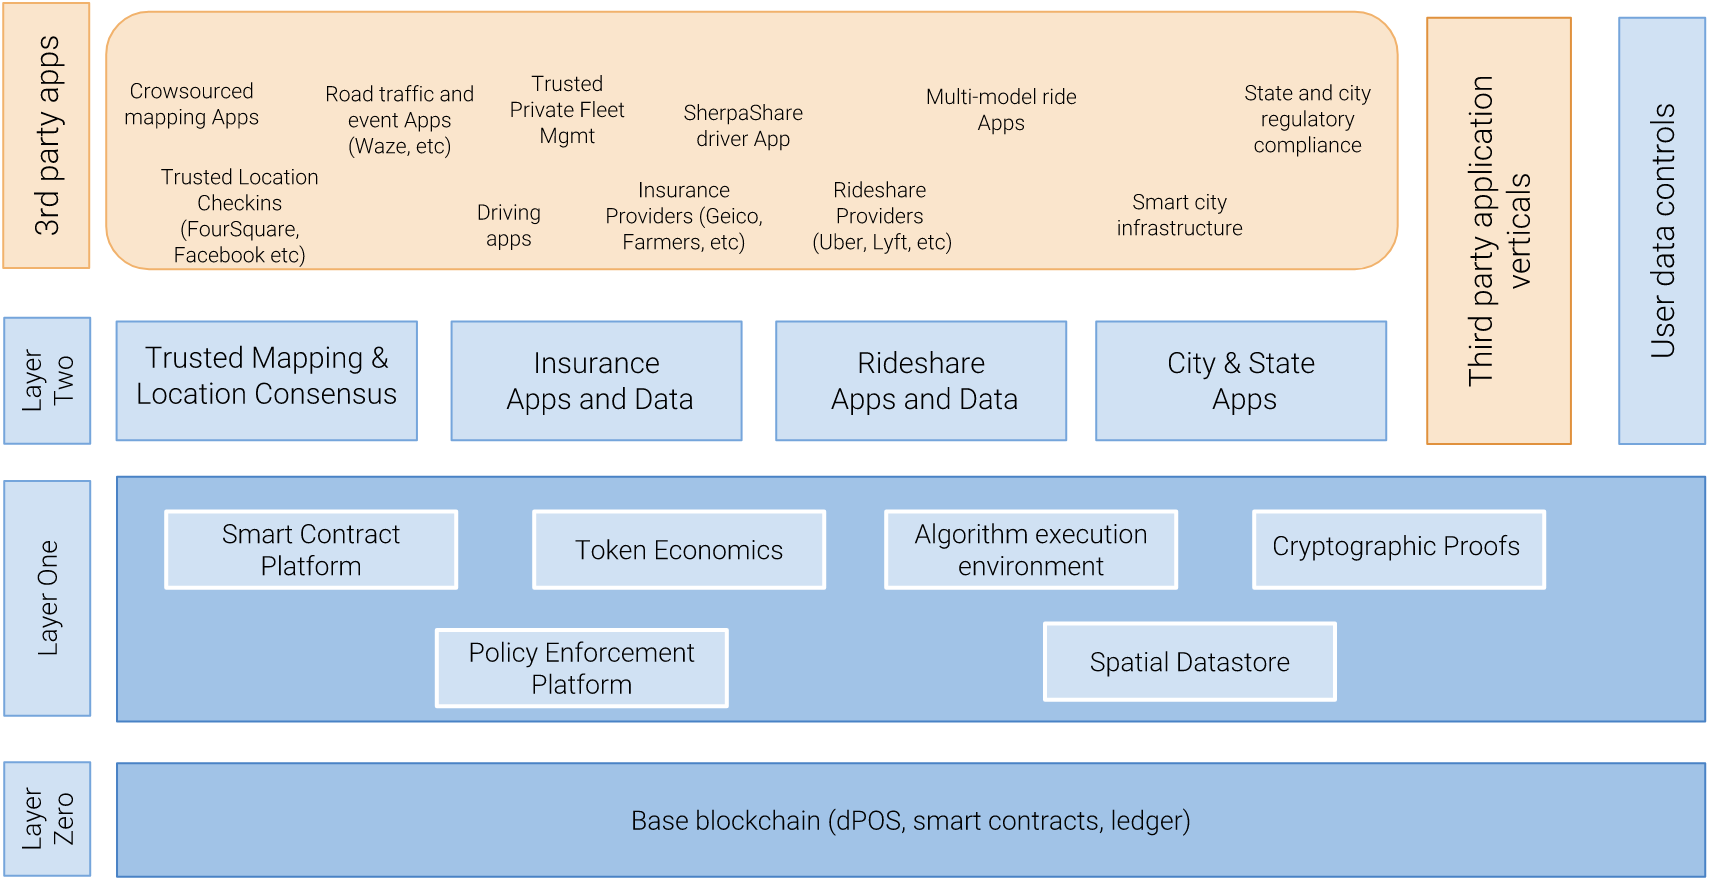
\includegraphics[width=1.00\textwidth]{lat-arch-2.png}
  \caption{Architecture of the Latitude Blockchain and associated platform ecosystem.}
    \label{fig:lat-arch}
\end{figure}

\section{The Latitude Platform}\label{sec:design}

In this Section, we present a high-level design of the Latitude platform. Latitude is a decentralized application
platform for Transportation. It is an application platform as it allows the development of applications in a
decentralized environment using blockchain technologies.

We start with an overview of the key design principles that will guide the rest of the design for Latitude. Its
important to note here that for implementation purposes, it might be possible to use an existing core blockchain for the
underlying functionalities and build Latitude as a layer on top. This is further discussed in Section \ref{sec:roadmap}.

Our goal is to become the best blockchain-based ecosystem in the world for decentralized applications for the
Transportation Industry. Specifically, Latitude can provide new ways to handle spatial, mapping, traffic, driving data
including data relating to other modalities of transport (bike sharing, walking, even air routes later on). Latitude
will provide novel methods to build applications that utilize this shared data.

\subsection{Architecture overview}
\label{sec:arch}

Figure \ref{fig:lat-arch} presents the architecture of the Latitude blockchain in terms of the core technological
innovations that will be built into it. The overall architecture of the Latitude Blockchain consists of a base
blockchain and a protocol implementation (Dapp SDK and smart contract APIs) for each application vertical. This choice
of an architecture gives the maximum flexibility for each application vertical to use its own protocol mechanisms for
token incentives while allowing for summaries or Merklized proofs of transactions to be commited to the base chain. In
the first (few) version of Latitude, the base chain might be an existing blockchain such as Ethereum, EOS, Zilliqa or
Neo. Eventually Latitude might move to a specialized design of a blockchain that works well for Transportation data and
dapps. The specific mechanisms for each business vertical shall be discussed in Section \ref{sec:apps}.

{\em Implementation Note:} For the alpha version of Latitude, it might be possible to use an existing chain with high
transaction velocity and low cost, such as EOS, Neo, Zilliqa or Harmony as a drop-in replacement for the base chain
functionality. In the long term, it might be beneficial to have our own base-chain with built in smart contract
functions for transportation applications. This will also work better with Latitude's own token economics. Further
discussed in Section \ref{sec:roadmap}.

{\em Side-chain based scaling:} As Latitude grows, it might be possible to transition each application protocol vertical
layer into its own side-chain. This will allow application-specific governence, consensus and contract rules to be baked
into the side-chain design. Depending on the application, it might be necessary for multiple side-chains to exist within
a vertical, in which case we shall use composable side-chains similar to Plasma. This allows for a hierarchical
side-chain structure if needed with eventual commitment to the mainchain. This is further discussed in Appendix
\ref{app:sidechain}.

\noindent {\em Base Blockchain layer (layer-0):} The Latitude platform uses a base blockchain layer for Layer-0
operations as shown in Figure \ref{fig:lat-arch}. The base layer can be an existing chain or Latitude's own blockchain.
For each application layer, Latitude provides middleware for layer 2 and 3 operations.

The base chain shall use Delegated Proof of Stake (DPOS) as its consensus mechanism.  DPOS is a fast, efficient and
decentralized consensus model available today. DPOS leverages the power of stakeholder approval voting to resolve
consensus issues in a fair and democratic way. All network parameters, from fee schedules to block intervals and
transaction sizes, can be tuned via elected delegates.  Deterministic selection of block producers shows that
transactions can be confirmed in an average of less than a second \cite{eos_producers}. This speed is important for
scaling the Latitude chain.

Latitude's DPOS system uses a set of "delegates" for voting on a block producer. The delegates are
"promoted" based on time-based trust or stake (or a combination of these). This design is similar to the Cosmos
blockchain and differs from other dPOS system such as EOS. The exact number of delegates can be a tunable parameter that
can be changed by the governing council of nodes. This version of takes the best of both cooperative and competitive
consensus algorithms.  The competitive part is larger stakeholders having an influence on their delegate of choice. In
Latitude, it is also possible to gain a larger stake by accruing what we call "trust" through honest operation over a
period of time. The delegates that have the most votes will take their turn to produce a block cooperatively in a
sequence. A $2/3$ majority of consensus among the delegates over the {\em last minted block} is needed to achieve
consensus and mint a new block onto the chain. Further discussion on Governance and other paremeters of a custom
Blockchain design are discussed in Appendix \ref{app:latchain}.

\subsection{Spatial datastore}
One of the central aspects of the Latitude blockchain is a geo-spatial datastore that fundamentally understands various
datatypes that are specific to transportation data. This datastore can use existing GIS databases that allow
de-centralized storage and access. The types of data include (i) geographic data such as location (latitude, longitude),
(ii) mapping data such as roads, terrain, addresses, etc, (iii) sensor data such as driving data, driver score, miles
driven, route information, etc, (iv) multi-modal transport data such as biking, walking and other means of transport.
Each of these data types have very special characteristics which the underlying datastore can be optimized for and allow
for programming using what we call the {\em Latitude Smart Contract} framework. 

The datastore would include spatial, quad-tree or an R-tree based indexes for efficient querying and other operations
that most Geographic Information Systems (GIS) would support in a centralized manner today. It would also include
functions to compute heatmaps, driving maps and statistics such as Traffic predictions including real-time analytics.
Depending on how Latitude evolves, the datastore can include additional functionalities to support the data sharing
among autonomous vehicles since they use most of the similar datatypes mentioned above. The datastore would support
circular, rectangular and other range queries, K-nearest neighbor searches, route optimization algorithms, etc. Figure
\ref{fig:geo_spatial_query} shows some of the queries that such a datastore can support.
For implementation purposes, Latitude shall use existing decentralized databases to support the spatial datastore
operations.

\subsection{Trust Ledger}
\label{sec:trust}

One of the core concepts in Latitude is the presence of a decentralized trust and reputation managment system. Trust and
reputation systems have been widely used in e-Commerce applications. They are well understood in terms of attacks and
game theoretic models \cite{rahimi_2017, rahimi_2012}. Latitude uses trust as a way to reward participants who have been
{\em consistently} honest over a period of time. Trust is also central in creating proofs on Latitude as discussed in
Section \ref{sec:crypto}.

The Trust ledger is a decentralized ledger accessible to everyone in the system. It consists of a trust model where each
participant's trust is stored and updated through specific operations. The following salient points explain the design
of the trust model in Latitude:

\begin{itemize}
    \item Trust is gained via honest operation: Each honest operation by a participant helps increase its trust value.
        The decision of whether an operation is completed honestly happens through consensus on a smart contract and
        depends on the specifics of an operation. For example, successful proofs of location or being a participant in
        proving other's location helps increase trust. As another example, reliable operation in contributing resources
        such as disk, network etc also helps increase trust.
    \item Trust is different from stake: Stake is purely a measure of the amount of LAT token held by an entity. While
        it gives economic incentives for entities to operate honest, it does not capture long-term honest operation
        behavior that Trust and Reputation system can do \cite{dong_2010}.
    \item Trust depreciation: Trust can depreciate either through dis-honest or unreliable operation. This decision is
        also arrived via consensus on an operation-specific smart contract. For example, if a participant contributes
        ride-sharing data which is shown to be flawed (possibly using a trusted party such as an Uber-API call),
        the trust level for this participant gets drained. Trust can also {\em decay} over time if nodes do not
        participate in network operations. Thus, there is a freshness dimension to the trust value in Latitude.
\end{itemize}

\noindent
{\em Half-life based exponential Trust decay:}
Trust in Latitude can decay over time in a way that is similar to how radioactive elements decay
using an half-life based formula shown below. This is to ensure that the trust values reflect freshness in operation.
The half-life value is a controllable parameter which indicates the duration after which the trust gets halved.
\begin{equation*}
    \label{eq_trust_decay}
    N(t) = N_0 \bigg(\frac{1}{2}\bigg)^\frac{t}{t_{1/2}}
\end{equation*}
where 
\begin{itemize}
    \item $N(t)$: The amount of trust at time $t$.
    \item $N_0$: The amount of initial trust before decay.
    \item $t_{1/2}$: Half-life of the trust decay model.
\end{itemize}

The amount of trust is used in Latitude to create proofs for various observations such as Location, Mapping, Traffic
etc. A combination of trust and stake are used in the DPOS and Governance operations.

Trust and Stake are combined into a single factor called the {\em l-factor}. The l-factor is computed as follows:

\newcommand\LFACTOR{\mathit{\text{l-factor}}}
\begin{equation*}
    \label{eq_l_factor}
    \LFACTOR(E) = \eta S(E) + \gamma T(E)
\end{equation*}
where
\begin{itemize}
    \item $\LFACTOR(E)$: The value of the l-factor metric for participant E.
    \item $S(E)$: The amount of stake put forth by participant E.
    \item $\eta$: Normalization factor for the stake metric.
    \item $T(E)$: The amount of trust as given in the trust ledger for participant E.
    \item $\gamma$: Normalization for the trust metric.
\end{itemize}

The l-factor value combines both trust and stake into a single metric which is used to determine if a node can be
allowed to participate in key network operations. These operations include block production, acting as delegates, or
even participation in the governing council.

\subsection{Cryptography layer} \label{sec:crypto} Latitude makes use of state-of-the-art cryptographic protocols to
provide various proofs, access control, confidentiality and other properties that are important in a decentralized
system.

such as AES encryption, secure hash functions, PKI certificates, multi-party key distribution protocols, proxy key
re-encryption schemes, Elliptic-curve based Digital Signatures \cite{ecdsa}. They help provide strong security, privacy,
access control, confidentiality and anonymity guarantees. Anonymity guarantees are an important part of data-sharing
smart contracts and privacy policies such as GDPR \cite{gdpr} especially for geo-spatial data such as location and maps.
Latitude provides anonymity guarantees using cryptographic set-preserving computations as derived from research in
\cite{kissner_set}. These can be suitably modified to allow for location-based anonymity which require stronger
guarantees when compared to set-based anonymity methods \cite{divanis_kanon,xu_loc_anon}.

Latitude also uses Merkle trees for cryptographic proof of audit, existence of data and verifiable computations
\cite{becker2008}. These proofs can be shared as certificates among participants or be used in the Latitude smart
contract system discussed later. They allow for verification of data existence or data-sharing contracts. They also
allow for the maintenance of a cryptographic log of all operations that happen on the network. These techniques are
similar to the ones used by some of the other blockchains today \cite{buterin_merkle}.

\subsubsection{Integrity and Access Control}

Latitude uses standard and well understood cryptographic protocols to provide robust access control and maintain basic
integrity of transactions. Data integrity is maintained using digital signatures. Every transaction is signed by one or more of the participants
certificates. The blockchain ledgers are protected using a Merkle hash \cite{becker2008} as discussed in the previous
section. A Merkle proof is used as a proof of transaction for cross-chain communication.

Access control for data that is not public or open, can be managed using multi-party key communication protocol (MPC)
\cite{enigma, nucypher, mpc_survey}. MPC protocols work over a set of $N$ trusted participants or a consortium set. They
can be designed to allow a minimum of $m<N$ participants to reach a consensus (using a off-chain protocol) in order to
compute the key that would grant access. Using these primitives, it becomes possible to have granular access control,
such as different amount of consensus for read, for writes and other semantic actions. Latitude shall make these
mechanisms available to the app developer through platform APIs. As always, since this is an open system, it is possible
for developers to build their own access control methods if they so wish.

%Cryptographic primitives for:
% - Security and privacy of data.
% - Anonymity guarantees using cryptographic set operations.
% - Enforcement of privacy when sharing data.
% - Sharing of “computation” instead of data when possible.
% - For eg: Sharing of DriverScore using a vetted algorithm.
% - Sharing proximity to a landmark instead of lat/lng.
% - Ability to find bad actors.
% - Detect privacy, anonymity and security violations.
%
%Cryptographic proofs for applications:
% - Proof of Location. 
% - Proof of ride. 
% - Proof of mapping 
%      (road/landmark exists or does not exist).
% - Proof of driver score 
% - Open, trusted, understood driver score computation algorithms.
% - Cryptographic proofs can be shared among entities, safely, securely.

In addition to these standard primitives, Latitude provides a host of other proofs that are tailor made
for geo-spatial, mapping, location and sensor data. These proofs can be used by applications, users and
other participants in the network. The network can be extended to create new forms of proofs as the application needs
grow. Below, we present the core set of cryptographic proofs that are unique to the Latitude blockchain:

\begin{figure}[t]
    \centering
    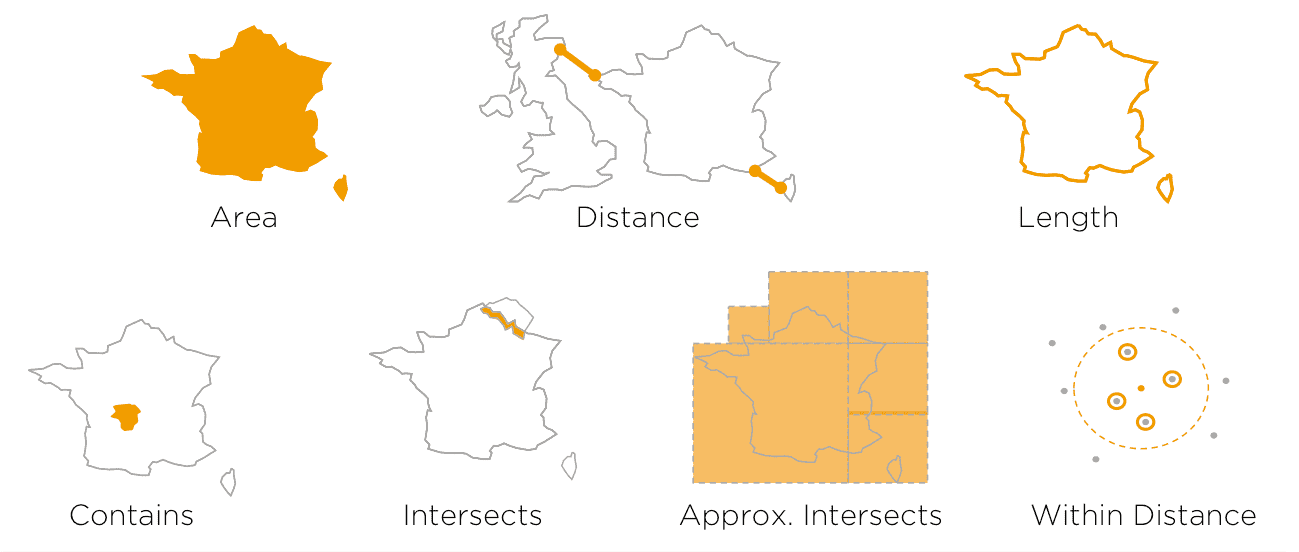
\includegraphics[width=0.70\textwidth]{geospatial_query.png}
  \caption{Examples of Geo-spatial queries that a spatial data-structure can support on the Latitude blockchain.}
    \label{fig:geo_spatial_query}
\end{figure}

\subsubsection{Proof of Real-world Observation}

A real-world observation could be a location computation, a ride from point A to B, a traffic observation or a landmark
at a given location. The core concept behind these observations is the flow of trust. The concepts presented in this
Section and the subsequent Sections replace and solve the offline Oracle problem that blockchains face today. These
mechanisms provide a practical method of creating a trust source of observation without requiring a perfect off-chain
Oracle \cite{concurrence}.

Any observation in the real world, be it a location or a landmark sighting is only as good as the trust placed in the
method and apparatus used to compute it. For example, if a GPS receiver returns a location, the amount of trust in that
location result is proportional to the amount of trust in the receiver construction and the satellite system being used
(such as Navstar, GNSS or others). Latitude uses this concept of trust as an internal metric to compute a proof of a
real-world observation.  Here we present the common algorithm used to compute these proofs which can be shared across
the Latitude platform.

\newcommand\NF{\mathit{Nf}}
\newcommand\TM{\mathit{Tm}}
\noindent
{\bf Definitions:}
\begin{itemize}
    \item Levels of trust $t_i, i \in \{0..M\}$, where $M$ is the max level of trust in the system. Trust level $t_{i+1} >
        t_i$.
    \item $t_0$ is the base level of trust assigned to any third party untrusted source of data.

    \item Each data source (such an an app installation, or a third-party source) is indentified using a certificate's
        public key. If this is a fully untrusted source that belongs to a third party, they start at the lowest level of
        trust $t_0$.

    \item $t_1$ is the trust assigned to a second party integration with Latitude's SDKs where the SDKs directly compute the
        observation and report it to the system using second-party APIs. Examples include Apps in the trusted App stores
        that integrate with Latitude.
    \item $t_2$ is the trust assigned to a first-pary integration, such as a Latitude mobile app, or a first-party app
        from trusted partners such as SherpaShare.
    \item $tmin_{pf}$ is the minimum trust needed for a specific proof or obervation. Each proof type might have a
        different requirment for this parameter. The computed proof also carries this parameters as an indication of
        consensus or trust.
    \item Trust map, $\TM(e)$ gives the amount of trust recorded in the ledger for the entity $e$. The entity could be an
        organization, an individual or a user (as identified by an app installation, for example).
    \item $N_{min}$ is the minimum number of entities that need to participate in the creation of this proof. This can
        be a function of the proof being created.
    \item The entity requesting the proof, submits a request $R(e, t_b, V, \TM(e))$, where $R$ represents the proof
        request. The request includes credentials for entity $e$, the base trust level in the request $t_b$, the
        evidence of real-world observation (such as radio signal strength) $V$ and the existing entry in the trust
        legder $\TM(e)$.
    \item Concurrence Weight: Each witness that concurs with an observation provides a {\em concurrence weight} which is
        the probability that they think the event happened. This is a value between 0 and 1. Denoted as $W_c(w, e, V)$,
        where the parameters are witness or observer $w$, entity $e$ and evidence $V$.
    \item Location specific trust normalization factor $\gamma_L$. $\gamma$ for a location $L$ is a location specific
        normalization factor which represents the average trust consensus in a specific location. For example, certain
        areas might have a higher concentration or honest or dishonest nodes. Or certain methods of location
        determination might have a bias that needs to be factored in.
\end{itemize}

Each proof is implemented as a special smart contract supported by the Latitude platform. The smart contract that
computed these proofs would provide a signed blob of data that certifies a certain observation as determined by the
respective proof.

\noindent
{\bf Algorithm for Proof of an observation $X$}:
\begin{enumerate}
    \item Suppose $e$ is the entity that initiates a request for proof of an obervation $X$ made by $e$.
    \item The proof system finds a subset (possibly randomly sampled) of participants $S$ who are able
        to {\it concur} with the obervation $X$. Each participant, $p_i \in S$, assigns a {\em concurrence} weight
        $W(p_i, X) \in [0,1]$ depending on how well they concur with the observation.
    \item Normalization factor $\NF(p_i, X)$: This is a multiplier, usually greater than 1, that signifies the
        amplification in trust as a funciton of how the observation was concurred upon. 
    \item Each observer $p_i \in S$, provides a normalization factor $\NF(p_i, X)$ and a concurrence weight $W(p_i, X)$
        to the proof.
    \item The proof computes the total trust in the observation $X$ as $T_{pf}(X, e, S)$, given by Equation
        \ref{eq_trust_compute}.
    \item Trust normalization: The total trust in $T_{pf}(X, e, S)$ gets normalized by $\gamma_L$ where $L$ is a coarse
        grained (city-level) location being considered. At bootstrap, a normalization factor of $1.0$ can be used.
\end{enumerate}

\noindent
Trust computation for a proof of observation X:
\begin{equation*}
    \label{eq_trust_compute}
    T_{pf}(X, e, S) = \sum_{i\in S} T(p_i) * \NF(p_i, X) * W(p_i, X)
    T_{pf}(X, e, S) = \gamma_L * T_{pf}(X, e, S)
\end{equation*}

where $T_{pf}(X, e, S)$ is the trust for the proof of observation $X$ proposed by entity $e$ and observed by
participants $S$. A proof is considered valid if $T_{pf}(X, e, S) > tmin_{pf}(X)$, that is, the accumulated trust is
above the minimum required for the type of observation $X$.

\noindent
Trust updates: Once a proof gets computed, the entity that initiated the observation gets its trust updated using an
EWMA formula. Assuming entity $e$ gets its trust updated for a proof $p_e$:
\begin{equation*}
    T(e)_{p_e} = (1 - \alpha) * T(e) + \alpha * T(p_e) / |S|
\end{equation*}

The goal of the above formula is multi-fold:
\begin{enumerate}
    \item To increase the average trust in an entity $e$ as a function of successful proofs. The larger the number of
        successful proofs, higher is the average trust in the entity.
    \item Similarly, the goal is also to reduce trust in case, with adequate participants, the system was unable to
        verify the claim. In fact, a larger draining of trust shall be instrumented if the system finds the claim to be
        demonstrably false.
    \item Malicious behavior: If an observer or the entity consistently disagrees with others in the proof system,
        over time their trust level will get degraded using a gradient method used in other reputation systems
        \cite{sen2010}.
    \item Rewarding honest behavior: Over time as observers and entities produce results with consistency, their
        historicla reputation gets better and recorded in the trust ledger.
\end{enumerate}

\subsubsection{Proof of Location:}

This is perhaps the most easily motivated functionality that the Latitude blockchain can provide. Proof of location is a
proof of real-world observation that proves that a given user, entity or participant is/was physically present at a given
location at a specific time. The location could also be relative to another participant or landmark.

Latitude shall provide the mobile, browser and sensor SDKs that can directly tie into the datastore to provide consensus
based proofs. These proofs can unlock applications such as access to facilities or help increase trust in crowd-sourced
mapping, traffic and incident reports.

The proof of location uses the above framework for a real-world observations with the following specification:
\begin{itemize}
    \item Entity $e$ computes a location on a mobile device. This could be an Android/iOS phone or a tablet/laptop.
        Depending on how the entity uses Latitude's SDKs, the location computation starts with a base trust level of
        $t_0$, $t_1$ or $t_2$.
    \item As a part of the location proof request $R(e, t_b, \TM(e), V)$, the entity can submit any evidence $V$ that would help
        prove the location. For example, on Android, this can include wifi-radio signals, cell tower signals, GPS
        satellite location and timing signals, Bluetooth-LE scans, and other signals that can help prove the location.
    \item Either the entity or the platform can find other participants for concurrence.
    \item Concurrence: A participant can concur by confirming the observations included in the evidence $V$. This can
        include, for example, a degree of concurrence or other factors that quantify how well they concur. The degree of
        concurrence can be a function of the radio signal properties \cite{mishra_secure, Mathur_2011}. This is used to
        compute the concurrence metric $W_c(w, e, v)$.
    \item Depending on the trust level of the observer, or for other considerations, the normalization factor can be
        used to boost or marginalize the contribution from a witness or observer $w$, denoted by $\NF(w, e, V)$.
    \item The witnesses or observers independently submit their recordings to the smart contract system, which either
        generates a valid proof or declines the request. At the end of each such operation, the new trust levels for
        various entities are computed.
    \item Historical Location: A past location proof from the same entity can be used as a "virtual observation" if the
        location computation is in the recent past. This combined with reasonable laws of Physics or motion can provide
        a small amount of trust for the current proof. For instance, if the entity was spotted at a grocery store about
        5 minutes in the past, then any new location update that is within a few miles of the grocery store could be trusted.
    \item Using the proof equation \ref{eq_trust_compute}, a trust level and proof is computed.
\end{itemize}

The location proof and the corresponding data including trust parameters are recorded in a web-friendly format (such as
JSON/XML) on a ledger specifically used for such proofs. The ledger entry can be used as a URL to refer to this proof
for other applications that can be built on top of it.

\noindent
{\em Other proof of location chains:}
The framework provided by Latitude is general enough to capture different implementations. For instance, \cite{foam}
uses a trusted set of radio beacons or "anchors" to provide location signals. These essentially become highly trusted
observers or participants in our framework as they are essentially first-party observers (with a large amount of
base-level trust). As another example, Platin is a blockchain designed specifically for a proof of location. Their use
of sensors and increase in trust over time falls in line with the general concept of proof of obervation (possibly with
different trust constants).

\subsubsection{Proof of Ride}

Provides a proof that a particular user has taken a ride from point A to point B using a
certain type of transport. This proof can be used across multi-modal ride platforms such as bike or car rides.  This can
be extended to include bus trips, flights, train rides and so on. The proof of ride credential will be available via the
Latitude mobile SDK on various platforms. Using the mobile SDK to construct these proofs also adds to the amount of
trust on the nature and parameters of the ride.  

The proof of ride is computed using a time series of location updates. A Hidden Markov Model or other methods
\cite{wu2011} can be used as "algorithmic observers or verifiers" of a location trace. The location trace can be
supplanted with sensor data collected using a direct integration of the Latitude SDK. The sensor data should be in full
correlation with the location trace and would consistute the evidence set $V$ for this proof.

The proof of ride algorithm is the following:
\begin{itemize}
    \item Entity submits an evidence $V$ which includes a series of locations, or proof of locations and sensor data.
    \item Platform can compute the trust as a function of trust inherent in included locatin proofs. Also, in certain
        cases, it might be possible to have other observers to correlate the ride (such as passengers or drivers in a
        rideshare scenario).
    \item Algorithmic observers such as physical properties of the ride can also be used to add trust to the system.
    \item Trusted observers: A small set of trusted observers such as API-based verification from Rideshare systems like
        Uber, Lyft and others can also be used as verifiers or concurrence providers to augment the proof.
    \item Depending on how well the observations correlate, the computed final trust is used to compute a proof of ride.
\end{itemize}

Proof of ride becomes a blob of signed data which gets recorded on the ledger.

\subsubsection{Proof of Landmark}

This proves the existence of a particular landmark such as a monument, a building, a sign post at a given lat/lng. This
can also be used to prove the existence of a particular road or the lack of. These proofs can be constructed using the
proof of location combined with consensus among users.  This proof can become the backbone for verified mapping and
landmark data-based applications.

The proof of landmark works as follows:

\begin{itemize}
    \item Multiple observers send evidence for a landmark. Evidence can include GPS-tagged photos or other sensor data
        (including 3D data of the area) using Latitude-integrated apps.
    \item Any observer or entity can request the proof. It might also
        be possible for the system to create a proof automatically based on sufficient collection of evidence.
    \item Based on the strength of individual observations, a smart contract can create such proofs.
\end{itemize}

The proof of landmark can be used for mapping and other applications in the Geo-spatial location and mapping industry.
These proofs can be stored on the ledger and in a spatial database which can make for efficient querying.

\subsubsection{Proof of DriverScore}

This proof can be computed on the blockchain over the data aggregated on the
datastore. The algorithm itself shall be made available to the nodes either as an executable docker image or an
open-source version. This allows different nodes to run the computation and create a certificate of driver score which
can then be attributed to the driver. This open framework can also allow different driver score algorithms to co-exist
in the system creating a community where better driver score algorithms can be agreed upon and used as the industry
standard.

A proof of DriverScore is computed as follows:
\begin{itemize}
    \item Driver score computation depends on the availability of open, trusted and benchmarked algorithms.
    \item The sensor data can be made available on a decentralized database or can run locally on the phone via
        integration with the Latitude SDK.
    \item The observers include location time series data that pass through HMM models for validation. For example,
        location and sensor data should make physical sense. Also they should be consistent with data from other
        drivers in the area in temporal proximity. Other validation includes co-riders in a ridesharing scenario. 
    \item Since this proof is very specific to each individual driver, it might take time for the system to be able to
        create enough trust in a single driver data report.
\end{itemize}

\subsubsection{Proof of Traffic}

Similar to the driver score, traffic is also an algorithm that looks at the statistics
of location and speed data on roads. The proof is similarly computed through consensus and recorded as a certificate on
the blockchain. The proof could be about real-time traffic or historic traffic patterns which can be shared with smart
city applications, the Census Bureau or other regulatory bodies.

Proof of traffic is computed as follows:

\begin{itemize}
    \item The traffic evidence consists of a location series including sensor data that can compute velocity,
        acceleration and other parameters. Usually a GPS location also includes a velocity vector.
    \item Proof of traffic can be computed by the system automatically upon gathering sufficient evidence from
        potentially unrelated observers or participants.
    \item Algorithmic verifiers will play a central role here as they are able to validate the traffic using time series
        location data, velocity vectors and correlation from multiple observers.
    \item Incident data which includes traffic incidents, constructions and other such events also can be part of this
        proof system and help augment the trusted in this proof.
    \item This is similar to a centralized traffic system such as one provided by Waze (or Google maps), except it is
        open, fully decentralized with the data available for any interested party to access.
\end{itemize}

\subsubsection{Proof of Route}

Similar to the functionality in the popular Waze app, this is about whether there exists
a certain route (or a better route) from point A to point B. More the consensus, higher the trust. For example, if a
user actually takes the route from A to B and provides a proof of ride, that helps create the proof of its existence.
This is useful for trusted and verifiable mapping / routing applications.

Proof of Route is computed as follows:

\begin{itemize}
    \item Just like a proof of ride, a proof of route consists of multiple location points in a time series.
    \item An algorithmic verifier, such as a HMM model could add to the validity of the route.
    \item Other observers could include participants who have also taken the same route at a recent times. These need
        not be ridesharing passengers.
    \item The Latitude platform, or an entity could propose a proof which can be executed upon sufficiently collected
        trusted evidence.
\end{itemize}

Proof of route can solve problems in mapping where the locals have the most up-to-date information on the routes, but
there is also an issue of trust. Major map providers such as Navstar, Google and others have way to crowdsource such
information with a reputation system in place to tackle malicious intent. Latitude's proof of route can solve this
problem to help provide reliable data for mapping applications.

\subsection{Latitude Smart Contract system}

\begin{figure}[t]
    \centering
    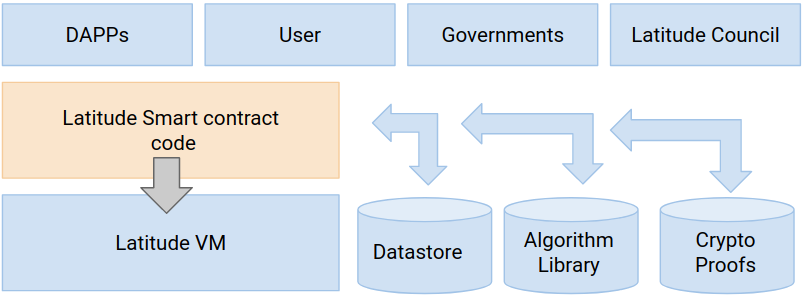
\includegraphics[width=0.60\textwidth]{lat_sc.png}
  \caption{Architecture of the Latitude Smart Contract framework.}
    \label{fig:lat-sc}
\end{figure}

Smart contracts are self-executing nuggets of code which specify the terms of the agreement between various participants
on the blockchain. For the Latitude blockchain, the participants can be a user, a regulatory body, an application
written by an insurance company or the city. The contract is directly written into lines of code in a certain smart
contract language. Popular smart contract frameworks today include ones used by Ethereum which runs on the Ethereum Virtual Machine (EVM),
the Neo which runs on the NeoVM and the EOS blockchain which runs on the WASM (WebAssembly VM).

The smart contract code and the agreements contained therein exist across the distributed, decentralized Latitude
blockchain network.  Because of this, Smart contracts permit trusted transactions and agreements to be carried out among
disparate, anonymous parties without the need for a central authority, legal system, or external enforcement mechanism.
They render transactions traceable, transparent, and irreversible as the state is always available on the Latitude
blockchain.

Figure \ref{fig:lat-sc} shows the high-level architecture of the Latitude Smart contract system. Latitude uses a
WebAssembly (wasm or eWasm) based compiler for a smart contract written in Go or C++. 

-- Overview of the webassembly architecture.

WebAssembly (or wasm) is a binary instruction format for a stack-based virtual machine. It includes a complier that is
portable and has a compilation target for high-level languages such as C++ and Go. The Latitude smart contract system
shall support both C++ and Go languages. The choice of wasm was to make the execution of the smart contract efficient
and thus have high throughput. Also, popular networks such as Ethereum are planning to move to eWasm as part of the
Ethereum Virtuam Machine (EVM) 2.0. This which will help create a common developer pool (and other aspects such as
tooling, educational material, etc) in the community. Wasm's execution happens in a safe and sandboxed
environment which can be beneficial in an adversarial and open network. It might also be possible to secure the Wasm
execution using Trusted Execution Environments (TEEs) in the near future.

The reason for chosing WebAssembly over the popular Solidity (or Vyper) used by the Ethereum Virtual Machine (EVM 1.0)
is twofold: 
WebAssembly compiles into native code and thus executes faster than Solidity or Javascript. Also, EVM 2.0 will feature
a modified version of WebAssembly, namely {\it eWasm} thus reducing the cognitive burden on developers across both
ecosystems.

Latitude uses a
modified version of Solidity (or the new Vyper programming language) as used by the Ethereum Virtual Machine. The choice
of this language is based on the production quality of the EVM, the language tools available in the community for
creating contract code, developer support and talent pool. Latitude shall add enhancements to the language to support
new spatial data types, indexes, cryptographic proofs and other mechanisms that are fundamental to the platform. Some of
the goals of the smart contract system include the ability to convert data policies such as GDPR \cite{gdpr} into
Latitude smart contract code which can then get automatically verified and enforced on the blockchain.  Also its
possible to share location data in an ephemeral manner for a specific purpose -- the data item gets automatically
destroyed using consensus and smart contract constructs on the blockchain. An example includes a user sharing their
location with an app for a very small duration of time.

As shown in Figure \ref{fig:lat-sc}, the smart contract code has access to the datastore, cryptographic proofs
(including algorithms to create proofs), an algorithm library (which hosts algorithms such as traffic, driver score
etc). These are directly accessible through language constructs making it easy to write high quality smart contract
code. The smart contract execution framework and related functionalities are accessible to dapps, entities such as
users, governments and the Latitude Council (discussed later in the Governance Section) on the system. 

The Latitude smart contract system can becomes the world's first such smart contract framework specifically tailored for
transportation data and applications.

\lstset{language=C++,basicstyle=\small}

\begin{lstlisting}[float, caption=Structure of a Latitude Smart Contract, frame=lines]

#include <latitude/contract.hpp>

// Shorthand for a location update that gets deleted in one hour.
typedef latitude::Location<TimeUnit<OneHour>> OneHourLocation;

class sample_contract : public latitude::Contract {

    private:
      // private data structures to the contract. The data does not go onchain.

    public:
      // data structures that can go onchain.
      // The contract methods will write to these.


      // There are two types of methods: Actions and callbacks.

      void onLocationUpdate(latitude::OneHourLocation curr) {
          // business logic
      }

      void computeProximity(OneHourLocation given, Location<NoExpiry> target) {
          // business logic
      }
}
\end{lstlisting}

\begin{itemize}

    \item Explain action methods.
    \item Data structures.
    \item Callback methods.
    \item Events.

\end{itemize}

\subsubsection{Secret contracts}

Typical smart contracts are public, including the data they operate on. For privacy or other reasons, it might be
desirable to achieve consensus on data without making it open on the chain. Latitude supports what are called secret
contracts using multi-party key distribution protocols. Multi-party key distribution creates a set of keys, such that a
function (or a smart contract) can be computed in a distributed manner over a random piece of data without any single
entity having full access to the data. The result of the computation has consensus and can be put on-chain using a
cyrptographic proof or can be directly communicated to a decentralized  app.

The availability of Trusted Execution Environments or hardware enclave can dramatically assist in the implementation of
secret contracts. In the first version of Latitude, we shall use existing MPC communication protocols in this area to
create a secret contract system similar to the one used in Enigma \cite{enigma}. In a later version, it might become
possible to use TEEs using a design similar to Ekiden \cite{ekiden}.

% Smart contract system for Transportation
% applications.  - Ability to convert “policies” such as GDPR into smart contract code.  - Example, self destruct data
% after a time period.  - Sandboxed trusted execution environment: - For algorithms: - DriverScore, Location heatmaps,
% Statistics.  - Enforcing or verifying privacy and other govt policies/regulations.


\subsubsection{Contract sharding}

Latitude smart contracts will be sharded to improve performance. Existing blockchains such as Ethereum, Neo and EOS
suffer from slow throughput on smart contract execution. One technique that has recently emerged as a way to scale
performance is to shard the contract using annonatations on methods to expose specific semantics. For example, by
understanding portions of a smart contract that store data, that verify computations and that are callbacks from
user-facing apps, it becomes possible to separate the execution among parallel nodes for much higher throughput
\cite{chainspace}. 

For example, in a given smart contract, certain data structures are annotated to store data. The dependencies between
the data structures is also specified as a group. There are three kinds of methods: Actions, callbacks and Verifiers. 
The Callbacks are used by the system to update the contract when a data or event happens, such as a user updates their
location. The Action methods are executed by the smart contract to take an action and the verifiers are methods that
verify transaction state. By isolating these methods and their data dependencies, one can shard a smart contract to
execute in pieces on different nodes on a blockchain thereby increasing efficiency and reducing the probability of a
coordinated attack.

Much like the other components, Latitude's smart contract sharding system shall leverage available algorithm libraries
and tools for rapid and iterative development.

\subsection{Token economics: The Latitude Token (LAT)}

Latitude has its own token for use on the Latitude Blockchain, called LAT. There would be a fixed token supply for a
certain period of time (4 years). A certain percentage of the tokens are reserved for funding and other operations, the
detials of which are not discussed in this document. The rest of the tokens will be available for the network. In this
Section, we discuss the Cryptoeconomics part of Latitude which creates the right incentive structure for various
participants.  For an overview of Cryptoeconomics in the blockchain space, please see \cite{sinclair_crypto}.

We shall use the work token model \cite{work_token}, where a certain number of tokens are pre-mind and ready for use.
The rest of the tokens can follow a transaction fee model, where the "miners" earn a certain fee for mining or minting
a block as per the consensus protocol. Out of 100\% tokens available for network operations, we shall have 70\%
pre-mined for network use and 30\% for block miners as rewards. The pre-mined tokens shall be used to subsidize network
resources, onboard the early adopters, fund developer communities, bug bounty programs and related activities.

The participants in Latitude are of the following types:
\begin{itemize}
    \item Miners: Anybody can "mine" the LAT token by contributin resources, such as disk, network and computing. This
        is similar to most other blockchains, which also allows Latitude to be built as a layer 1-3 stack on other
        chains for the first few versions. The miners earn transaction fees and token rewards for mining a block. The
        consensus protocol is dPOS as discussed in the earlier Section.
    \item Users: Users who contribute data can be rewarded using the LAT token. They usually contribute using a partner
        app such as a Ridesharing app. They can subsequently convert the token into other uses on the platform or into
        fiat.
    \item Data providers: These could be institutions that transact on Latitude to provide transportation data. The data
        could be modified to reduce any privacy loss and could purely be sensor or raw mapping/location data. The
        availability of proof of X would increase the trust in the validity of the data.
    \item Data consumers: These are participants such as insurance companies or ad-networks who can consume
        transportation data. They could consumer real-time data, such as real time ride sharing information for a
        certain city. Or it could be aggregate data for deep learning algorithms.
    \item Dapp developers: These are developers who build apps on the Latitude platform. They would purchase data,
        capacity or other features of the platform on a per-transaction basis. Deep discounts and other incentives can
        be used to seed this community.
    \item Regulators: These are government agencies who implement policies on the transactions in any given industry.
        They can use the LAT token to implement and execute such policies as code on the platform. They can also
        institute fines using the token or create incentives structures for honest players.
\end{itemize}

The salient features of the Latitude token economics are the following:
\begin{itemize}
    \item Assume greedy but honest participation: The miners are incentivized to produce blocks through honest operation
        using the dPOS consensus mechanism.
    \item Users and data providers are rewarded for contribution of data. The actual reward and verification happens
        through smart contracts. For example, in a Waze-like application, users are rewarded for posting accurate
        traffic incident information. These are a key component of the token economics and we discuss this in further
        detail below.
    \item Data sharing for deep learning, such as computing driving score or other mechanisms gets incentivized using
        the token.
    \item Deposit draining: Stake and deposit are drained if malicious operation is suspected. This is implemented using
        smart contracts for any data sharing. This technique is also used for dPOS consensus operations.
\end{itemize}

%Latitude shall employ a Proof of Stake model (delegated or non-delegated) for participation and core node-level mining. This mechanism has recently
%gained popularity among a notable number of blockchains \cite{dpos_steemit}. This also allows for deposit slashing as a
%technique to tackle Byzantine behavior. Latitude will employ techniques such as Minimal Slashing \cite{buterin_slashing}
%for Byzantine fault tolerance and safety under distributed asynchronous operation.

\noindent
{\bf User incentives:}
Token economics allow for the creation of what we call user incentives. These are protocol constructs in the blockchain
that allow users to benefit from the value they create for the ecosystem. Refer to \cite{token_ecos} for an overview on
incentive mechanisms to reward users for various methods of participation in the network. In general, the Latitude token
ecosystem will be based on market economics, that is, supply and demand from various participants will be the primary
driver for prices and incentives in the network. This philosophy falls in line with decentralized control and operation
while also allowing for creating most reward for honest behavior in the network.

The ability of user incentives to exist in a decentralized manner can be disruptive to existing incumbents in the
sharing economy space, such as Uber, Lyft, Airbnb, etc since users can get rewarded in a tangible manner for their
contributions \cite{sharing_eco_bc}. Consumers shifted to apps in the sharing economy as they provided cheaper and
better alternatives to traditional services like Uber and Airbnb. However, since all transactions go through these
centralized providers, the platform owners determine the fees, percentages and are in complete control of any data
practices and policies which cannot be verified. They often become accused of predatory behavior. Using blockchain based
incentives, sharing and open-source software these problems can be addressed in a singular fashion.

As an example, consider the Ridesharing application. As users contribute data on what rides they are taking, it becomes
possible for the network to reward them with tokens. They could, upon sufficient contribution, redeem them for free
rides or share with them others on the network. A similar model can be adopted for data concerning driver behavior where
drivers using different apps and sensor algorithms can elect to share their data towards building a better driver score
in return for suitable incentives.

\noindent
{\em Token mechanics: Based on the above design, we discuss the various ways in tokens get exchanged on Latitude:}
\begin{itemize}
    \item Mining: Nodes can earn tokens when blocks are mined using the DPOS algorithm discussed in Section
        \ref{sec:arch} and Appendix \ref{app:dpos}.
    \item Transaction fees: Transcation fees help pay delegates and DPOS participants for transactions. These could be
        block production transaction or proof of X. For the proofs, the transaction fees are shared by the network and
        the other participants regardless of whether a proof succeeded or failed. Also, for each smart contract
        execution, the transaction fees get paid to the nodes that act as verifiers and to the network.
    \item Security deposit (or collateral): Nodes put up stakes in order to participate in the voting process or the
        Governing council. These stakes are in the form of the LAT token.
    \item Dapps: Dapps built on the Latitude platform will transact on the LAT token. This could include datastore
        resources, compute, network, proof of X or other SDK integrations.
    \item Application specific business model: For each of the specific application areas such as Telematics or
        Ride-sharing, there will exist specific models for transacting tokens. These shall be discussed in their
        relevant sections.
\end{itemize}

\subsection{Governance on Latitude}

Governance refers to a decentralized manner in which decisions are made using a consensus mechanism on the blockchain.
Decisions include basic constructs whether a node can join or leave the network. Or it can include key decisions on
whether an upgrade should be mandated on every node, a given participant such as a data provider should be penalized. It
could also include issues where humans get involved, such as when a user complains of a loss of privacy or a breach in
contract.

Recently blockchains have been moving towards governance using a small set of participants, such as trusted miners in
the case of Stellar and Ripple \cite{stellar_gateway}. The EOS blockchain uses a similar concept of a core set of block
producers who are elected based on a nomination and voting process \cite{eos_producers}. For discussion around
Governance in Ethereum, refer to \cite{buterin_gov}. Latitude uses a similar concept of a {\em council} of participants.
These are entities (nodes or organizations) that have demonstrated participating using earned trust through honest
operation, accumulating stake, demonstrated good intent and establishing trust. Some members of this council might
include the core Latitude developers which allows them to implement operations such as updates, bug fixes and so on. The
council members shall be elected using the an election protocol on the blockchain. It might be possible to directly
nominate certain council members such as regulatory bodies who have general interest in user rights, privacy and
enforcement. 

% - Crypto-incentives for honest operation.
% - Penalties for malicious intent.
% - Governance based on consensus and roles using a council.
% - Council members elected using voting, stake and established trust.
% - Some council members can have restricted access.
% - Eg: US govt can have voting rights on US data/users, etc.

The operations of the Governance council happen in the following manner:
\begin{itemize}
    \item Nodes that accumulate sufficient l-factor credentials and have been involved in block production or other
        operations for a certain amount of time can be nominated by the network to be part of the council. 
    \item Council membership is dynamic. Every participant has to demonstrate continued honest operation, trust and
        stake in the network. This makes it democratic and open.
    \item Council decision process. Governance decisions are created by council nodes and require a high amount of
        approval from all such members. Examples include, changing voting parameters, proof of X smart contracts,
        decisions on updates to rule (to reduce forks) and other governance rules. The handbook of governance contracts
        shall be created once the Latitude testnet is stable and ready.
\end{itemize}

\begin{figure}[t]
    \centering
    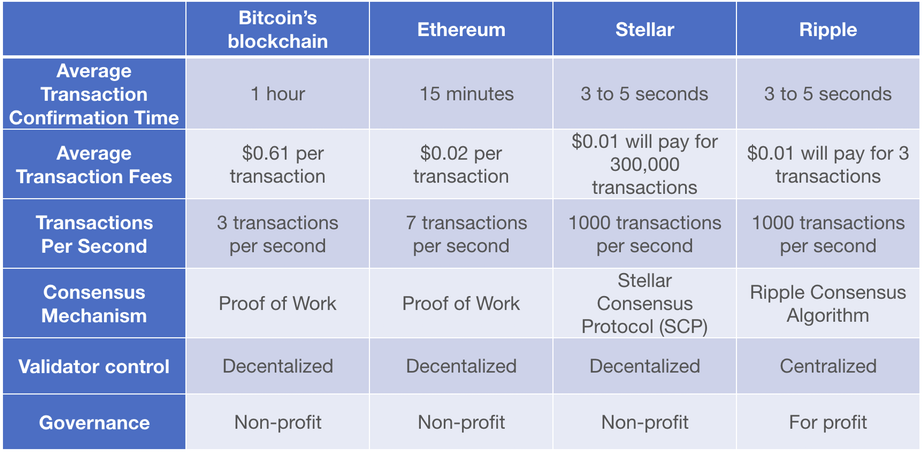
\includegraphics[width=0.90\textwidth]{tps_speed2.png}
  \caption{Comparison of transactions per second of the major blockchains today.}
    \label{fig:tps_speed}
\end{figure}


\section{Application Sidechains}
\label{sec:apps}

In this section, we discuss the four different classes of applications that can be built on the Latitude platform. Each
of these applications is supported by a suite of software modules, smart contract add-ons and SDKs (mobile and desktop)
that utilize the core functionality offered by Latitude and provision it in unique ways to suit the specific class of
applications. Each application is a side-chain that posts its aggregated transactions to the main-chain if needed.
The Latitude platform is extensible in the sense that its not limited to these four classes of
application side-chains. For example, its possible to add additional applications such as for the shipping or the airline industry
as verticals on the platform. Next we discuss each of these applications and how they can be supported on the platform.

\subsection{Ride-share application side-chain}

Ride-sharing applications are the pinnacle of the applications in the data sharing economy. They empower the user to
choose from a multi-modal ways of finding or providing rides. Latitude can provide the decentralized infrastructure to
store, share and build decentralized applications for their corresponding counterparts.

The ride-sharing market alone is large enough to power the Latitude blockchain as its primary use-case. The ride-sharing
market is around 17 Billion dollars with around 60 Million users. This does not include the multi-modal ride sharing
segment which is growing rapidly. This segment includes bike, scooter and such modes of transport. The ARPU is around 
293 dollars which is high enough to create user incentivized models for data sharing. The data generated by these users
currently sits in silos in the respective ride sharing apps, which can be unlocked and put to good use through such
mechanisms. 

Latitude shall provide a mobile SDK and a blockchain API specifically to suit ride-sharing apps for sharing data. This
would allow the creation of decentralized ride sharing apps that can provide users with incentives to share data,
subsidize rides and provide a better deal for ride providers. They can also allow regulators to enforce the use of
roads, lanes, parking and other structures in accordance with city or neighborhood ordinances. Latitude's SDK shall also
provide a multi-modal ride API that such apps can use to request rides on the platform.

As an preferred third-party integration, Latitude shall integrate with SherpaShare's platform for drivers. This would
allow greater sharing of the geo-spatial and driving data collected through SherpaShare's driver app. This will be one
of the early launches for the beta version of the Latitude platform.

%Overview of ridesharing applications. Big industry leaders. Statistics on rides, miles, revenue, ARPU.
%
%Multi-modal ride data:
% - Bike, scooter ride apps.
%Disruptive to Bikesharing:
% - Mobike, OFO, BlueGoGo, Youon, Mingbikes
% - Hellobike, YooBike, CCbike, Zagster, LimeBike
% - Citi Bike, Capital Bikeshare, Divvy, Hubway, Docomo Bike
%Share, Relay Bikes
% - Public transit data
%Use SDK/app to share data. Similar incentive model.
%Monetization:
% - Single multi-modal ride API (SherpaShare or 3rd party).
%
% Ridesharing platform:
%
% Platform:
%Latitude Ridesharing SDK.
%Ridesharing sidechain on the Latitude blockchain.
%Riders:
%Contributing ridesharing data:
%Uber, Lyft, Gett, Juno, Curb, Sitbaq
%Drivers:
% - Use SherpaShare app or 3rd-party app with SDK.
% - Proof of ride:
%Using driver-side app and/or client app.
%Other players:
% - City, Law enforcement, analytics use cases.

\subsection{Telematics side-chain}

Data is the most important asset for Telematics applications. Thus, sharing of data, computations and algorithms can be
beneficial to companies, users and the ecosystem in general. In fact, by using the Latitude blockchain it becomes
possible for regulators to enforce laws better while maintaining data privacy. This can result in lower crime rates and
incidents.

The important of data sharing here can be seen from the existence of {\em Telematics data exchanges} that are
centralized cloud-based exchanges which act as data brokers among users and insurance companies. As an example, consider
the Verisk Data Exchange (verisk.com) which allows the exchange of driver data to insurance companies. They share data
for all kinds of connected vehicles for underwriting, rating, and claims handling through Usage-based Insurance (UBI)
programs.  The exchange stores and processes Telematics data of all types, volumes, and velocity from connected cars,
after-market hardware, or mobile solutions. A second example is the Octo Telematics company which also operates an
exchange that is used by over 100 insurance companies, has about 186 billion miles of driving data and gets 11 billion
new data points from 5.4 million connected cars and sensors every day.

The problem with such centralized solutions is that there is a central entity that extracts the fees and has direct
control over the data. Such centralization can result in security and privacy loss and lack of trust from all parties
involved. Latitude is directly poised to disrupt this market by providing a blockchain based platform for exchange of
data, computation, algorithms and resulted information. Using Latitude smart contracts it becomes possible to enforce
proper security, privacy and sharing of data in accordance with agreed upon incentives. This implies cleaner and better
sharing methods which can be a win-win for everyone in the industry including the regulators.

Latitude shall provide a Telematics SDK and blockchain library module to enable such applications. This would include a
suite of pre-existing smart contracts, datastore provisions and other software modules necessary to build decentralized
data exchanges which can eliminate the expensive data brokers. The SDK shall also include APIs for Usage-based Insurance
companies to act as data providers given appropriate involvement, permission and incentives for the users. Users can
also be incentivized to provide data directly to the platform by getting token rewards. Such a model also allows for
open experimentation with driver behavior algorithms such as DriverScore. It also becomes possible for drivers and users
to "carry" their score or reputation from one platform to another, thus preventing lock-in scenarios.

%---Telematics data sharing:
%Data sharing can result in better algorithms, better understanding among drivers.
%Telematics data can save lives:
%Allows government regulations to be enforced. Data privacy can be enforced.
%Driver’s own their driving history (score) and can choose to carry it.
%
%
%---UBI methods can be improved with data sharing and incentives.
%Example:
%Octo telematics
%20 million miles, 186 billion miles of driving data
%100 insurance companies (data is not shared).
%11 billion new data points daily from 5.4 million connected cars and sensors.
%Disruptive opportunity for data sharing.
%
%
%
%---Telematics data exchanges exist today !
%But centralized, unclear policies, enforcement.
% Lack of control.
% Example: Verisk Data Exchange (verisk.com)
% The first-of-its-kind  exchange draws driving data from all kinds of connected vehicles for underwriting, rating, and
% claims handling through UBI programs. 
% The exchange is scalable to normalize, process, and store telematics data of all types, volumes, and velocity from
% connected cars, after-market hardware, or mobile solutions.
% Finally, one exchange solves the many-to-many challenge by connecting auto-makers and telematics service providers
% (TSPs) to multiple insurers
%
%
% ---Insurance Vertical
% Latitude Driver SDK:
% Allows trusted capture of driving data.
% Platform for running DriverScore / Behavior algorithms on phone or in the cloud (or a combination). 
% Eg: Geico:
% Can run 3rd-party algorithms such as Geico’s driver score directly on the phone.
% Includes API for interacting with Geico’s app.
% Users mine currency by:
% Contributing driver data, driver scores.
% Users own the data, have full control.
%
% Insurance providers (Geico, Progressive, Farmers, etc)
% Use platform for computing metrics.
% Contribute data/and or crypto-currency incentivized.
% Always user permissioned.
% Other players:
% City, Law enforcement, analytics use cases.
% Car history use cases (better version of Carfax).

\subsection{Mapping and Location side-chain}

Mapping and Location-based services and analytics is another big segment that Latitude can address through
decentralization. Mapping and real-time location/speed data is a huge market that apps like Waze are able to access.
However, the user incentives in Waze are limited to the Waze platform and cannot be carried over. Finally, the data that
users contribute also stays isolated to the Waze platform and cannot be used by the City or the National Transportation
Safety Board (NTSB) for altruistic purposes. To get a sense of the market size, today Waze has about 70 million users
with 500K volunteers who provide real-time data. A Waze user on average spends about 480 minutes per month on the
platform.

The Latitude blockchain can change all of data isolation and platform lock-in by providing strong incentives to the user
by rewarding them with crypto-currencies. The smart contract system can also be used to enforce proper sharing of data
with the right participants. The built-in primitives in Latitude for Byzantine behavior can be used to ensure honest
operation at all times.

Location-based services can be similarly decentralized on Latitude. Using the mobile Latitude SDK, it becomes possible
for users to directly contribute mapping and location data to the platform. This allows Latitude to construct the
various cryptographic proofs as discussed in Section \ref{sec:crypto}. Proof of location technology alone has the
potential to disrupt the "Check-ins" industry. The Facebook platform alone gets about 50 million check-ins per year. The
other major players here include Foursquare, Yelp and Google maps. The sharing of check-ins data on the Latitude
platform can enable new applications not previously possible due to the platform lock-ins.

%Waze example:
% - 70 Mil users, 500k volunteers share data. user spends 480 min/month.
%
%-- Upcoming mapping applications include:
% High-resolution data for self-driving technology.
% Road data, needs consensus and trust.
% Proof of location:
% Location enabled maps. 
% Foursquare checkins. Facebook checkins.
% Location-based access control.
% 3 BILLION location requests daily on Android
% 250M location-enabled service users.
%
%--Latitude Mapping + Location SDK
%Mobile SDK for trusted mapping + location.
%SherpaShare app + 3rd party apps.
%Users mine by:
%Contributing road, traffic, street, mapping data.
%Contributing user location
%Proof of location concept can replace “Check-Ins”
%Facebook has 50 million check-ins per year.
%City, law enforcement, analytics use cases.
%User has full privacy control.
%
%-- Applications:
%Waze like apps:
%By Latitude Mapping/Location Sidechain.
%Waze, OsmAnd, Maps.Me, HEREWeGo, 2GIS
%Yandex.Maps, Locus Maps.
% Navmil, NavIt, MapQuest.
% Crowd-sourced maps.
% Authenticated location applications:
% Access control or privileges by virtue of location.
%
\subsection{Smart city and Govt Application side-chain}

Smart cities refer to a large set of applications that can improve the life of a citizen by providing better amenities.
Examples include real-time data for parking, data-driven urban planning, city-wide zoning research,
environmental location sensors, disaster management, transport/transit data (real-time and historical), smart transport
(shuttle/bikes), traffic light management to name a few.

Latitude blockchain can host such smart city applications and collect data from their citizens. Users are incentivized
to provide data using token economics and the regulators or city officials can "purchase" data or results using smart
contracts. It might be possible to share aggregated data with careful focus on privacy/anonymity to State level or
Federal government for various regulatory reasons. 

%One of the final set of applications.
%Smart city applications:
% - Parking, data-driven urban planning, waste management, water software and analytics, environmental location sensors,
%   disaster management, transport/transit data (real-time and historical), smart transport (shuttle/bike),
%   connectivity citywide, grid/energy, traffic light management, security and survelliance.
%
%  Users mine by contributing data.
%  Govt requests access using crypto.
%  Use cases:
%  Census, traffic, analytics, city-wide zoning research.
%  Real-time understanding of citizen data.
%  Compliance:
%  Insurance, Ridesharing companies regulatory compliance enforced using smart contracts on the Latitude blockchain.


%\input{mech}

\section{Conclusion}
\label{sec:conc}

Blockchains have the potential to disrupt incumbent applications on the data sharing economy. In addition to this, the
Transportation industry is going through a radical shift due to the new types of data and applications that have become
available. For instance the proliferation of mobile phones has brought a surge in crowd-sourced data. Also widespread
deployment of cheap hardware sensor networks combined with smart analysis and planning algorithms are able to utilize this
data to create valuable new insights and applications that were not previously possible.

By bringing the blockchain technology and designing it from the grounds up for Transportation applications, we have created
the world's first blockchain specifically tailored for Transportation applications. Our mission is for Latitude to become
the de-facto platform for all transportation applications by building the right constructs for trusted, privacy-aware,
secure and verifiable data and computation sharing/enforcement.

Latitude shall support applications across the planet and across different modes of transport. We
are excited by how Latitude stands to disrupt existing applications such as Ride-sharing, Mapping, Location sharing and
analytics and the driver-behavior industry (UBIs).


% One section per vertical.

% Core blockchain aspects. Smart Contract system. DataStore etc.

% Governance. Consensus, cryptoeconomics.

%-----------------------------------------------------------------------------
%  OVERALL DESIGN SECTION
%-----------------------------------------------------------------------------
%\input{design}

%----------------------------------------------------------------------------- BIBLIOGRAPHY
%-----------------------------------------------------------------------------

%\section{Team}

Latitude has a highly competent team with a 20+ years of combined experience in the areas of location, ride sharing, mapping and
geo-spatial technologies. They have built some of the widely used products in the Industry today in these areas. They are well suited to take this plan to a successful execution.
\newline
\newline
\noindent
{\bf Jianming Zhou:}
Jianming is the CEO and co-Founder of SherpaShare, the leading driver assistant app to help ridesharing drivers to
maximize their earning potentials. He has more than 12 years of experience in the location industry. He was the founding
member of Alohar mobile(acquired by Alibaba group) and built the first Telematics engine used by MileIQ (acquired by
Microsoft). Previously, he was the engineering director at Loopt, the pioneer service in the mobile social local space
founded by Sam Altman. Before that, he was the engineer at Telenav which built the first turn-by-turn navigation system
on mobile devices. He holds an MS degree in Computer Science and majored in P2P network security and privacy.
\newline
\newline
\noindent
{\bf Tony Qin:}
Tony is AI Research Lead at DiDi Research America.  He established the reinforcement learning research at DiDi Chuxing
from scratch.  Previously, he was Staff Data Scientist at Walmart Labs.  Tony is an experienced and accomplished
scientist with a research background that intersects AI, machine learning, and optimization.  He has built numerous
successful AI and machine learning-powered solutions for ride-sharing and E-commerce domains.  He holds a Ph.D. in
Operations Research from Columbia University and has more than 15 conference and journal publications, 9 US patents, and
many more pending US and international patents.  He is an editorial board member and reviewer of various research
conferences and journals, and most recently, Senior Program Chair of AAAI 2019.
\newline
\newline
\noindent {\bf Colin Jia Zheng:}
Colin is the software engineer at Google working on distributed database system. He
holds a Ph.D degree in Computer Science from Harvard University and major in Cryptography.
\newline
\newline
\noindent {\bf Chanjun Yang:} Chanjun is the tech lead at Google Data Infrastructure Team. She has a MS degree in
Computer Science from ISU and a BS from Peking university. 
\newline
\newline
\noindent
{\bf Andrew Pillsbury:}
Andrew Pillsbury is VP Business Development for SherpaShare where he is responsible for B2B partnerships and sales. Previously he has held executive roles at The New Yorker Magazine and Macrovision (pre and post IPO). He has an MBA from The Wharton School and a BA from Duke University.
\newline
\newline
\noindent {\bf Jennifer Israel:}
Jen Israel is a passionate marketer with experience in integrated business to consumer marketing - brand, product,
marketing partnerships, customer relationship marketing, CPG and digital. Before joining SherpaShare as Head of
Marketing, Jen spent six years in fin-tech at Green Dot Corporation as the GoBank Mobile Bank Account brand and product
marketing leader directing strategic marketing planning, development, and execution.  Jen was responsible for launching
the first mobile bank account to be sold in Walmart, and the successful Uber Visa Debit Card, growing the program to
over 100,000 customers in the first year.
\newline
\newline
\noindent {\bf Arunesh Mishra (advisor) :} Dr. Mishra has 10 years of research and development experience in the Industry in
Location and Mapping. At Google, he built the Location platform used widely on Android and Chrome and Google Maps
applications. He was the core designer for the crowd-sourced algorithms that self-learn and power the location/mapping
for Google's mobile platform. The platform serves more than 2 Billion users daily. He holds a PhD, 30 issued patents and
22 pending patents today many of which are based on the physical layer mechanics of computing location and mapping. He
was won Best Paper awards at top ACM conferences and has over 30+ conference publications. He has widely contributed to
open source software used on standard Linux distributions today. He has also built the largest mobile peer-peer network
infrastructure for iOS/Android via Google Play Games offering.


\section{References}
\bibliography{fullwp.bib}

\newpage

\begin{appendices}

\section{Why use a Blockchain ?}\label{sec:blockchain}

In this Section, we go over the key reasons why a Blockchain-based platform is the right solution for Latitude. We
start with an overview of the Blockchain technologies and present the pivotal features that would work well for the
business use case of Latitude.

Blockchain has the potential to become the new decentralized application platform for the Internet. Blockchain is a
public register in which transactions between two users belonging to the same network are stored in a secure, verifiable
and permanent way. The data relating to the exchanges are saved inside cryptographic blocks, connected in a hierarchical
manner to each other. This creates an endless chain of data blocks -- hence the name blockchain -- that allows one to
trace and verify all the transactions they have ever made.

The introduction of Bitcoin \cite{nakamoto2009bitcoin} triggered a new wave of decentralization in computing.
Bitcoin illustrated a novel set of benefits: decentralized control, where ``no one'' owns or controls the network;
immutability, where written data is tamper-resistant (``forever''); and the ability to create \& transfer assets on the
network, without reliance on a central entity.

The initial excitement surrounding Bitcoin stemmed from its use as a token of value, for example as an alternative to
government-issued currencies.  As people learned more about the underlying blockchain technology, they extended the
scope of the technology itself (e.g. smart contracts), as well as applications (e.g. intellectual property).

Bitcoin was the first such blockchain to introduce the concept of full decentralization, but Ethereum has made this a
general platform for executing arbitrary applications called dapps using smart contracts and a wide range of other
tools. Since Ethereum, there has been an explosion in blockchain technology to allow a wide range of distributed
decentralized applications to run over a network of untrusted arbitrary nodes over the planet, which almost mimic the
structure and spread of the Internet.

%Blockchain is a
%public register in which transactions between two users belonging to the same network are stored in a secure, verifiable
%and permanent way. The data relating to the exchanges are saved inside cryptographic blocks, connected in a hierarchical
%manner to each other. This creates an endless chain of data blocks -- hence the name blockchain -- that allows you to
%trace and verify all the transactions you have ever made.

 The primary function of a blockchain is, therefore, to certify transactions between people. In the case of Bitcoin, the
 blockchain serves to verify the exchange of cryptocurrency between two users, but it is only one of the many possible
 uses of this technological structure. In other sectors, the blockchain can certify the exchange of shares and stocks,
 operate as if it were a notary and "validate" a contract or make the votes cast in online voting secure and impossible
 to alter.

Decentralization is one of the core concepts or features of a blockchain. It can mean different things in different
contexts but for our purposes it allows for two important things:
\begin{itemize}
    \item Decentralization of control or power: That is, no single entity such as a company or an institution has
        unrestricted control over all aspects of the data. In a centralized world, for example, Uber has direct control
        over all user data and how that data is being shared with third-parties, etc. Of course, there are privacy
        policies that are published, but as a user one has no choice but to place full trust in the policy or their
        implementations. There is no method of open verification or recourse in case of a breach. With a
        blockchain-based solution, all participants on the network have equal say. Using primitives such as consensus
        and smart contracts, it becomes possible to verify and enforce such policies.
    \item Decentralization of software: There is no single centralized place on the Internet which hosts the
        functionality or the data. The blockchain itself is stored in a decentralized manner on the nodes that form the
        network and thus, there is no single point of failure or trust associated with the system. This is a big
        advantage that blockchain systems have over centralized solutions.
\end{itemize}

As a result of this decentralization, the blockchains get some nice benefits as given below:
\begin{itemize}

    \item Fault tolerance - decentralized systems are less likely to fail accidentally because they rely on many separate
components that have uncorrelated failure models.
    \item Attack resistance - decentralized systems are more expensive to attack and destroy or manipulate because they lack
sensitive central points that can be attacked at much lower cost than the economic size of the surrounding system. This
can be important for transportation data as it does not remain under a single point of failure.
    \item Collusion resistance - it is much harder for participants in decentralized systems to collude to act in ways that
benefit them at the expense of other participants, whereas the leaderships of corporations and governments collude in
ways that benefit themselves but harm less well-coordinated citizens, customers, employees and the general public all
the time.
\end{itemize}

One of the key concepts of blockchains becoming an application platform is smart contracts. A standard contract, as a
legal document, binds two or more parties into an obligation to achieve certain deliverables or outcomes. A smart
contract is a piece of code that similarly binds multiple parties into outcomes that are verifiable, computable or
provable using code and strong cryptographic constructs. Ethereum was the first such platform to introduce the concept
of smart contracts which has since been adopted by most other blockchains that wish to host decentralized applications
(dapps).

Because smart contracts can be executed by arbitrary nodes on the blockchain, its possible for anyone to "verify" the
smart contract. This creates the concept of trust using consensus. Consensus is defined as the agreement among a
certain number (or fraction) of nodes on a particular result or outcome. With consensus, it becomes much harder for a
Byzantine or adversarial node \cite{lamport_byz} to manipulate the smart contract in ways that was not intended or
provisioned for. One of our goals, as discussed later in Section \ref{sec:design} is to build a smart contract framework
that is tailored for Transportation applications, so that the contracts are readily available, trustable and
enforceable. 

Smart contracts can allow new ways of data sharing that were not possible before. By creating strong programmatic
constructs combined with consensus protocols and cryptographic primitives it is possible to share data in a way that
privacy, security and restrictions on use can be enforced. There has been a lot of recent progress on how to use Smart
Contracts for data sharing \cite{liu_2018}. Thus, the technology today is ready for creating disruptive new ways of
sharing transportation data to create new applications such as smart cities, driver behavior, insurance, mapping etc.
This technology can be disruptive to incumbents who might be late for adoption.

Blockchain software is generally open-source. This increases the trust level to what is not possible in centralized data
silos.  Open source software removes the need for policies to exist in text, but can be verified in code. Also it allows
anyone in the community or the industry to contribute to functionality thereby moving the industry towards
standardization which is good for the ecosystem. This makes it possible for the Industry or Government to create
regulations or an industry standard and also implement a method of enforcing them on the network.

%- Concepts of smart contract, trust, consensus.
%
%- How data sharing can work in a blockchain manner. 
%- Overview of cryptographic proofs. How they work.
%- Discussion of Byzantine behavior.
%
%-Blockchain based Platform is decentralized.
%    - No single point of control or failure.
%    - Users own their data and reputation.
%    - Every functionality is openly verifiable.
%
%- System is open-source
% - Every entity knows how data, algorithms and logic is implemented.
% - Policies can be verified using Trusted Computing.
%
%- Anyone can participate including Governments, Individuals, Enterprises.
%- Governance happens using a council of participants.
%- Privacy and Security policies can be enforced through strong cryptographic primitives.
%
%
%- Smart contracts allow for precise enforcement of incentives, data sharing and privacy protection.
%- Industry or Government Standards are enforceable and verifiable.
%- Raw and derived data can outlive the companies or geographies.
%- Eg: DriverScore can carry over to a different country or geography.
%- Mapping data can be utilized outside of the GIS provider.
%
%


\newpage
\section{The Latitude DPOS Consensus Algorithm}
\label{app:dpos}

Latitude uses the Delegated Proof of Stake algorithm for consensus. This method allows honest participants and stake
holders to partake in block production. The same philosophy is also used for electing the Governance council. All
operations are transparent and any participant can become part of such operations through honest commitment to the
system.

Like other PoS chains, DPoS doesn't include miners who run hashes to produce blocks. Instead, an elected subset of
participants is chosen to perform the work of validating the chain. These participants are called block producers,
delegates, notaries, validators, forgers, or witnesses. DPOS or variants thereof is being widely used in the blockchain
space, current blockchains utilizing DPoS include:

\begin{itemize}
\item EOS, BitShares, Steem, Golos, Ark, Lisk, PeerPlays, Nano (formerly Raiblocks), and Tezos
\item Cosmos/Tendermint, Cardano, and a few others use consensus algorithms loosely based on DPoS
\end{itemize}

Latitude uses a combination of stake (amount of LAT token held as collateral) and trust (value in the trust ledger as
discussed in Section \ref{sec:trust}. The block production algorithm works as follows:

\begin{itemize}
\item Participants who own a certain amount of trust and stake are allowed to act as delegates. Trust and stake are
    combined into a single metric called the l-factor as given in Equation \ref{eq_l_factor}.
\item Delegates can choose to nominate block producers. Their vote is weighted by their l-factor value. The block
    candidates who receive the most votes are elected to be block producers. Users can also delegate their voting power
        to others on their behalf. Thus DPOS creates a representative democracy with stake and trust based suffrage.
\item The number of block producers is lower bounded $N_{min}$ and upper bounded $N_{max}$, but is not a strict value.

\item Block producers can be voted out any time if bad behavior is determined. The threat of loss of stake and/or
    reputation is a deterrent to bad behavior. Also slashing conditions can be easily implemented if so desired.
\item Block consensus: Once a block producer set is determined, a consensus algorithm such as PBFT is used to
    achieve $2/3 +1$ majority to decide on a block. Producers always converge to the longest chain as as long as a
        majority of the block producers are honest, the system will converge.
\item Block production time: This can be set to a desirable value, such as 0.5 or 1 second to make it periodic.
\end{itemize}

DPoS doesn't attempt to 'find' a balance between the number of block producers needed to ensure that control is
sufficiently decentralized and the number of block producers that can easily be monitored for bad behavior. Rather, it
explicitly sets the balance, though it can be modified later through governance protocols.

\noindent
{\em Rewards for block production:} While some blockchains such as EOS, purely reward block producers through inflationary
economics, Latitude uses a combination of transaction rewards and inflation. The rewards allow nodes that demonstrate
trust (and less stake) to earn tokens. The exact distribution of reward vs inflation based earnings shall be determined
via experiments and research on the testnet.

\noindent {\em Scalability of the consensus algorithm:}

Known and limited block producers (delegated nodes or participants) means that blocks can be propagated through the
network much more efficiently, enabling significant scalability increases. Blocks can also be consistently and reliably
produced in a much smaller time frame. Also by tuning various parameters, it becomes possible to set this timeframe to
as low as 0.5 seconds if desired.  Furthermore, finality can be reached as soon as $\frac{2}{3}$ of the block producers have
confirmed a transaction, with strong guarantees that a transaction is on a valid chain even before that. 

Given that the top 5 blockchains, in terms of speed, are using DPOS, this becomes the natural choice for Latitude.

\newpage
\section{Scaling the Latitude Architecture}
\label{app:latchain}

As the Latitude platform grows both in terms of aggregate data/users or partners, it might become necessary to split
each application vertical into its own side-chain. A Latitude base-chain will work with various side-chains to enforce
basic platform rules such as governance, token pricing, platform-wide smart contracts, etc.  

Each side-chain is essentially its own blockchain with Merkle summaries being committed to the main chain. This
side-chain architecture can be used to accomplish the following:

\begin{itemize}
  \item Side-chain specific Governance: It becomes possible to divide governance into application specific rules on
        each side-chain. For example, a ride-sharing side-chain could include governance rules specific for ride
        providers and consumers. In a Telematics side-chain, the governance could include rules on how new driver
        behavior algorithms are benchmarked, etc.  For example, open deep learning algorithms that compute DriverScore
        can be required to demonstrate their performance on a public dataset available on the chain. Changes to these
        algorithms might require higher level of consensus and demonstration of performance.

  \item Scaling operations: Side-chains allow Latitude to scale operations by only committing chain-wide state changes
      to the main-chain. These include account balances, core council or trust operations to be committed to the main
        chain, allowing all other application specific transactions to stay limited to each side-chain.
   \item Representation of Users: The side-chain could include rules the directly empower users to control their data.  The definition of a
user could be an entity that contributes driving data using one of the SDK-integrated apps.  Users can be directly
represented as special entities on the chain in a separate ledger that lists them. These concepts shall be fully
developed at the point when Latitude scales enough to warrant a side-chain based design.

  \item Permissioned or Enterprise side-chains: Side-chain architecture also allows Latitude to offer a permissioned,
      consortium or enterprise version. This looks more like a standard SaaS model where a set of companies can lease
        service space on the Latitude chain for their consortium operations.
\end{itemize}

\subsection{Side-chain mining}
In general, we expect the side-chain mining to use variants or the same DPOS mining algorithm as the main Latitude
blockchain.  However, the design allows for each side-chain could potentially have their own mining or consensus based
block reward algorithms. For example, the ride-sharing sidechain could reward users for sharing data. Certain
permissioned side-chains could potentially use their own token which converts to the Latitude token on the main chain.

Certain side-chains, such as the smart-city applications might purely operate on a proof of work model and eliminate
mining altogether.
\begin{figure}[t]
    \centering
    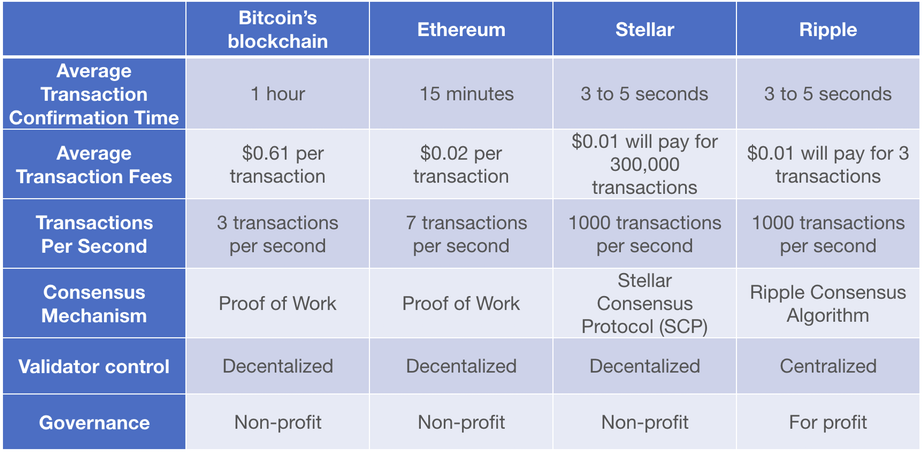
\includegraphics[width=0.90\textwidth]{tps_speed2.png}
  \caption{Comparison of transactions per second of the major blockchains today.}
    \label{fig:tps_speed}
\end{figure}
\subsection{Differentiated Consensus}
When thinking of performance, one of the key metrics that is hotly debated in the community is transactions per second.
Bitcoin is know for its long time to produce a block, on the order of minutes which limits the number of transactions
the network can process. Figure \ref{fig:tps_speed} shows a comparison of the major blockchains today with respect to
this crucial metric. Note that these blockchains shown in the Figure are primarily evaluated against the concept of a
transaction which represents a transfer of assets, goods or monetary value digitally on the blockchain. Stellar and
Ripple are two blockchains that have gained popularity for financial transactions as they tout a higher transaction
velocity. 

In the context of Latitude, the performance of the blockchain is important. The blockchain will handle different types
of data and transactions which will require different levels of consensus and trust. Figure \ref{fig:tps_lat} shows the
different types of transactions that the Latitude blockchain can process and the performance we expect to achieve.

Latitude uses the concept of {\em Differentiated Consensus} to scale to a higher transaction speed. The amount of
consensus depends on the transaction type and the possible Byzantine attack scenarios. We next discuss each type of
transaction and how trust/consensus would work for them:

\subsection{Datastore transactions}
These refer to basic transactions to store data values into the geo-spatial data
store. For instance, if a user shares their driving data, this can include the sensor information, lat/lng of the trip
taken and any mapping data collected. For ride-sharing applications, this can include any multi-model ride details that
the user has booked. We expect the blockchain to be able to process close to 1-10 million transactions per second, since
most such transactions require very low level of consensus and can tolerate eventual consistency \cite{eventual_con}.
These transactions are essentially database CRUD transactions, with each request containing enough credentials to
warrant low consensus. The credentials can include access control signatures for a permissioned table, or proofs of X
which handle the offline oracle problem for consensus. Thus, basic database-level Paxos consensus can be used for such
transactions to ensure high velocity. 

\subsection{Algorithm executions}
These refer to transactions which include executing known algorithms on the blockchain. For instance, this could include
the computation of various driver behavior algorithms with the computation being shared among certain participants on
the network. Another computation could include statistics such as real-time traffic or aggregate traffic statistics
shared with a city for better zoning and planning purposes. The amount of consensus required is relatively small but
higher than datastore operations in order to ensure correct execution of algorithms and lack of malicious intent. Also
such operations would require strong consistency for their CRUD functionalities. We expect the Latitude design to
support 10-100K transactions per second at its peak usage.

These transactions essentially use the computing resource on the network. The consensus is achieved through verifying or
using a small set of testdata for each algorithm. The verifier nodes are randomly chosen and paid for using the
transaction fees. Depending on how much consensus is needed, the smart contract responsible for the algorithm execution
can lock in certain amount of token as collateral (or escrow).

\subsection{Data sharing contracts}
These transactions refer to the creation, deletion or arbitration of long-term sharing smart contracts between
participating entities. For instance, it could include a new contract between an insurance company and a data provider
for sharing certain types of driver score data for certain geographic locations. Since these transactions have higher
value they require larger amount of trust and consensus in the system. Latitude shall support a transaction speed of
around 100-1000 transactions per second for this category.

The consensus required is generally high for such transactions due to the monetary value and long-term impact on the
participants. We expect all such transactions to go through the full consensus on the blockchain and get recorded on the
main chain. DPOS consensus should be able to support the required transaction speeds. 

\subsection{Governance operations}
The Governance operations require the highest amount of trust and full consensus of the network. These include voting to
add/remove council members, critical council decisions such as forks or updates/upgrades, decisions on high-value smart
contract disputes, etc. The transaction velocity is low for reasons of trust, accuracy and correctness and thus we
expect the Latitude blockchain to support 1-10 transactions per second under this category.

\subsection{Storage capacity}
Another metric of importance for Latitude is the storage capacity in the network. This can be important for
datastore operations. We expect the storage capacity, network bandwidth and any other computing resource to become
available on an incentivized model as determined by usage contracts. For instance, if a user is willing to share data with
a data consumer, the consumer should be able to allocate token resources to provision the network with sufficient
storage. The token can be used to purchase storage using other blockchain storage providers such as Filecoin, Siacoin or
Golem can be used to incentivized nodes to directly supplant on-chain storage.

\begin{figure}[t]
    \centering
    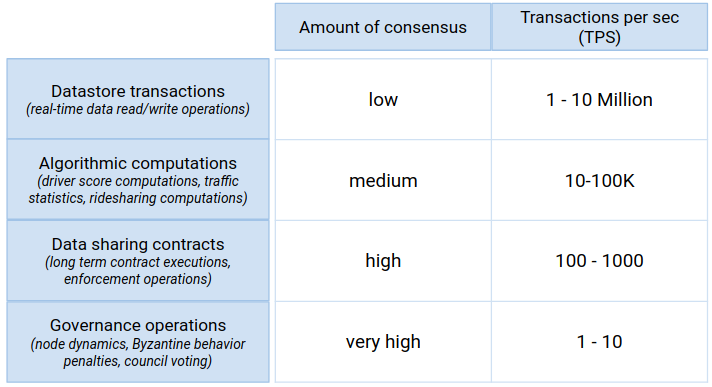
\includegraphics[width=0.75\textwidth]{tps_lat2.png}
  \caption{Expected Transaction per second velocity of various types of functionalities on the Latitude Blockchain.}
    \label{fig:tps_lat}
\end{figure}



\end{appendices}


\end{document}
